\input{../header_1_en.tex}




\usepackage{Sweave}
\begin{document}

\begin{frame}[allowframebreaks]
  \titlepage
\end{frame}

\section*{Class outline}

\begin{frame}[allowframebreaks]
  \frametitle{Basic microarrays}
  \tableofcontents[hideallsubsections]
\end{frame}

%%%%%%%%%%%%%%%%%%%%%%%%%%%%%%%%%%%%%%%%%%%%%%%%%%%%%%%%%%%%%%%%%%%%%%%%%%%
\section{Intro}

\begin{frame}[allowframebreaks]
  \frametitle{About}
  \begin{itemize}
  \item On this short class we'll learn how to do linear regressions, correlations and use the limma package.
  \end{itemize}
\end{frame}

\begin{frame}[allowframebreaks, fragile]
  \frametitle{Session packages}
  \begin{itemize}
  \item Install commands:
\begin{Schunk}
\begin{Sinput}
> install.packages("UsingR")
> source("http://bioconductor.org/biocLite.R")
> biocLite(c("limma"))
\end{Sinput}
\end{Schunk}
  \end{itemize}
\end{frame}

\section{Linear regressions}

\begin{frame}[allowframebreaks]
  \frametitle{Quick intro}
  \begin{itemize}
  \item The idea behind a linear regression is to fit a line to a given data set. This line will try to pass through the center of the data, such that the data points are close.
  \item Once you have the linear regression you can predict values :)
  \item There are a lot of methods of linear regression models, but we'll take a look at the simplest one.
  \end{itemize}
\end{frame}


\begin{frame}[allowframebreaks]
  \frametitle{Basic linear regression}
  \begin{itemize}
  \item Basic equation:
  \begin{equation}
  y_i = \beta_0 + \beta_1x_i + \epsilon_i
  \end{equation}
  \item Here, $\epsilon_i$ is the error, $\beta_0$ and $\beta_1$ are the regression coefficients, $x$ is the independent variable \& $y$ the dependent one.
  \item In statistics, we generally know $x$ but need to estimate the rest.
  \end{itemize}
\end{frame}

\begin{frame}[allowframebreaks, fragile]
  \frametitle{Functions}
  \begin{itemize}  
  \item In \pl{R} we can do some simple linear regressions using \BIOCfunction{lm (model.formula)} where we use \pl{y TILDE x} for the formula. For example:
\begin{Schunk}
\begin{Sinput}
> library(UsingR)
> res <- lm(homedata$y2000 ~ homedata$y1970)
> res
\end{Sinput}
\begin{Soutput}
Call:
lm(formula = homedata$y2000 ~ homedata$y1970)

Coefficients:
   (Intercept)  homedata$y1970  
    -1.040e+05       5.258e+00  
\end{Soutput}
\end{Schunk}
  \item Instead of just calling \pl{lm}, its better to save the resulting object. Then we can use this object to plot it or obtain more information with functions such as:
  \begin{itemize}
    \item \BIOCfunction{coef} gives us the coefficients
	\item \BIOCfunction{residuals} to find the residuals
	\item \BIOCfunction{predict} to predict a value for a given $x$
  \end{itemize}
  \item \alert{Note} that linear regressions are not meant to predict values outside the valid range for your independent variable ($x$).
  \item Sometimes its useful to transform your data so that the linear model will be more appropriate. For example, log transform the data.
  \item Some other linear regression functions which are more resistant to outliers are: \BIOCfunction{lqs} and \BIOCfunction{rlm}.
  \end{itemize}
\end{frame}

\begin{frame}[allowframebreaks]
  \frametitle{Plotting the lm object}
  \begin{itemize}
  \item How would you plot the linear regression? Its a line :)
  \end{itemize}
\end{frame}

\begin{frame}[allowframebreaks, fragile]
  \frametitle{With \pl{abline}}
  \begin{itemize}
  \item Its not with \BIOCfunction{lines} but with \BIOCfunction{abline}: \scriptsize
\begin{Schunk}
\begin{Sinput}
> args(abline)
\end{Sinput}
\begin{Soutput}
function (a = NULL, b = NULL, h = NULL, v = NULL, reg = NULL, 
    coef = NULL, untf = FALSE, ...) 
NULL
\end{Soutput}
\end{Schunk}
  \item \normalsize Now plot the data and the regression line :)
  \end{itemize}
\end{frame}

\begin{frame}[fragile, allowframebreaks]
  \frametitle{Plot}
\begin{Schunk}
\begin{Sinput}
> plot(homedata$y1970, homedata$y2000)
> abline(res, col = "red", lwd = 2)
\end{Sinput}
\end{Schunk}
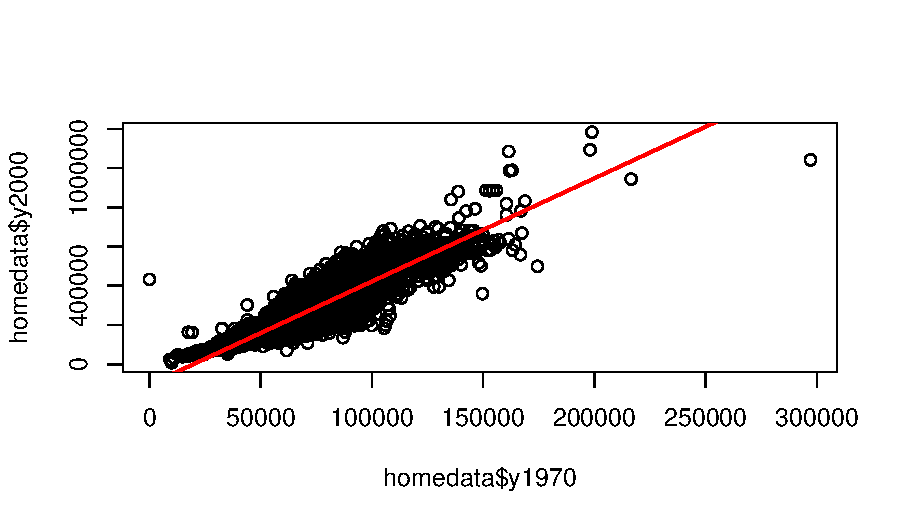
\includegraphics{plots/fig-005}
\end{frame}

\begin{frame}[allowframebreaks, fragile]
  \frametitle{Exercise}
  \begin{enumerate}
  \item Using the \pl{kid.weights} data frame, make a plot of weight vs height).
\begin{Schunk}
\begin{Sinput}
> head(kid.weights)
\end{Sinput}
\begin{Soutput}
  age weight height gender
1  58     38     38      M
2 103     87     43      M
3  87     50     48      M
4 138     98     61      M
5  82     47     47      F
6  52     30     24      F
\end{Soutput}
\end{Schunk}
  \item Transform one of the variables to make the plot better.
  \item Re-make the plot with the transformed variable.
  \item Do a simple linear regression.
  \item Plot the line from your resulting lm object.
  \end{enumerate}
\end{frame}

\begin{frame}[fragile, allowframebreaks]
  \frametitle{Part 1}
\begin{Schunk}
\begin{Sinput}
> plot(kid.weights$weight ~ kid.weights$height)
\end{Sinput}
\end{Schunk}
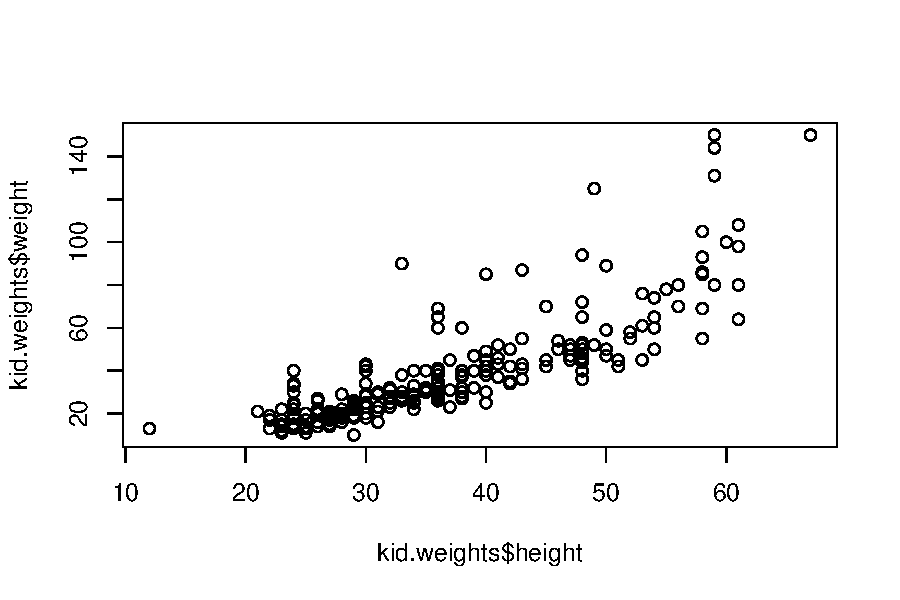
\includegraphics{plots/fig-007}
\end{frame}

\begin{frame}[fragile, allowframebreaks]
  \frametitle{Parts 2 and 3}
\begin{Schunk}
\begin{Sinput}
> height.sq <- kid.weights$height^2
> plot(kid.weights$weight ~ height.sq)
\end{Sinput}
\end{Schunk}
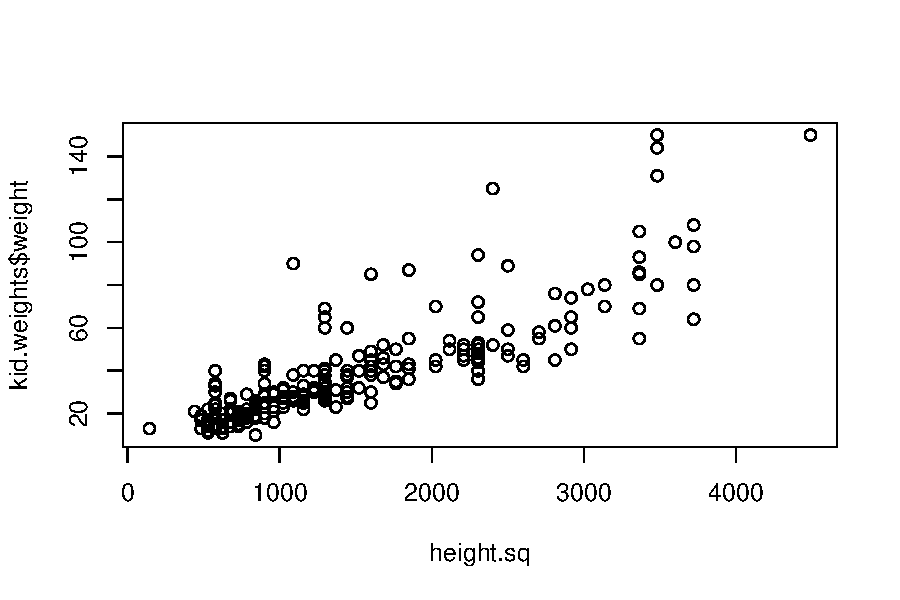
\includegraphics{plots/fig-008}
\end{frame}

\begin{frame}[fragile, allowframebreaks]
  \frametitle{Parts 4 and 5}
\begin{Schunk}
\begin{Sinput}
> height.sq <- kid.weights$height^2
> res2 <- lm(kid.weights$weight ~ 
+     height.sq)
> plot(kid.weights$weight ~ height.sq)
> abline(res2, col = "blue", lwd = 2)
\end{Sinput}
\end{Schunk}
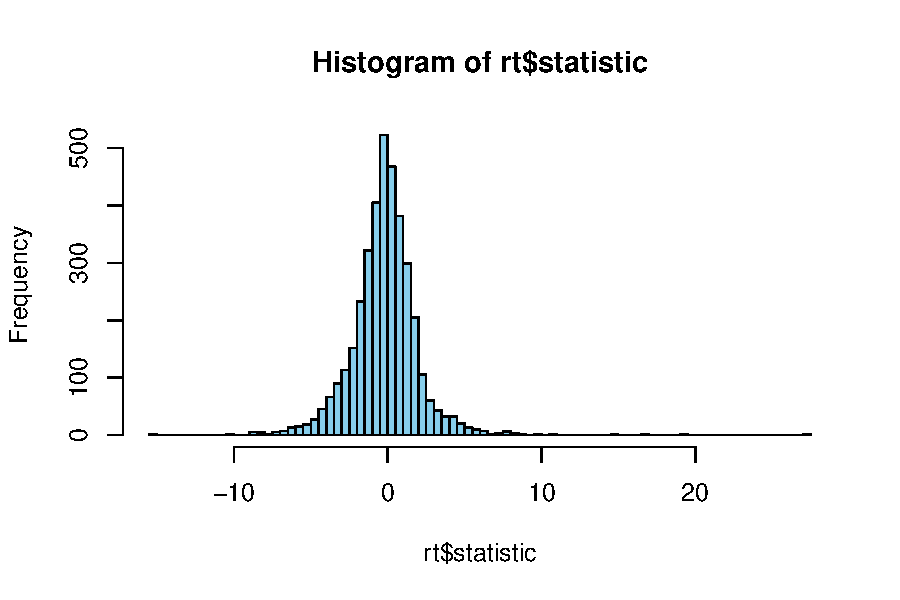
\includegraphics{plots/fig-009}
\end{frame}

\section{Correlations}

\begin{frame}[allowframebreaks]
  \frametitle{Correlations}
  \begin{itemize}
  \item Many times when you have two variables you'll want to know if they are correlated. A correlation as taken by \myurlshort{es.wikipedia.org/wiki/Correlación}{wiki esp}:
  \begin{itemize}
    \item \emph{indicates the force and direction of a linear relationship between two random variables. Two quantitative variables are considered to be correlated when the values of one of them varies systematically with respect to the homomin values from the other one: if we have two variables (A and B) there is a correlation when the values of A increase so do the values of B and viceversa. The correlation between two variables doesn't imply, by itself, any relation of casuality.}

  \end{itemize}
  \item In \pl{R} we can find the coefficient of the Pearson and Spearman correlations easily.
  \end{itemize}
\end{frame}  

\begin{frame}[allowframebreaks, fragile]
  \frametitle{Pearson correlation}
  \begin{itemize}
  \item It tells us how correlated are two variables.\footnote{Its independent of the scale of the variables.}
  \item For more information, check \myurlshort{en.wikipedia.org/wiki/Pearson's_correlation_coefficient}{wikipedia}.
  \item In \pl{R} we can find the Pearson correlation using the function \BIOCfunction{cor}:
  \end{itemize}
\begin{Schunk}
\begin{Sinput}
> cor(homedata$y1970, homedata$y2000)
\end{Sinput}
\begin{Soutput}
[1] 0.8962155
\end{Soutput}
\begin{Sinput}
> cor(maydow$max.temp[-1], diff(maydow$DJA))
\end{Sinput}
\begin{Soutput}
[1] 0.01028846
\end{Soutput}
\end{Schunk}
\end{frame}  

\begin{frame}[allowframebreaks, fragile]
  \frametitle{Spearman rank correlation}
  \begin{itemize}
  \item This one is useful if the relationship between the two variables is not lineal, but increases. More info at \myurlshort{en.wikipedia.org/wiki/Spearman's_rank_correlation_coefficient}{wiki}.
  \item To use this one, we need to order the data from smallest to biggest into ranks. We can do so using the function \BIOCfunction{rank}: \scriptsize
\begin{Schunk}
\begin{Sinput}
> args(rank)
\end{Sinput}
\begin{Soutput}
function (x, na.last = TRUE, ties.method = c("average", "first", 
    "random", "max", "min")) 
NULL
\end{Soutput}
\end{Schunk}
  \item \normalsize In \pl{R} we can calculate this correlation using \pl{cor(rank(x), rank(y))} or simply using the argument \pl{method} from the \pl{cor} function.
\begin{Schunk}
\begin{Sinput}
> cor(rank(homedata$y1970), rank(homedata$y2000))
\end{Sinput}
\begin{Soutput}
[1] 0.8878185
\end{Soutput}
\begin{Sinput}
> cor(maydow$max.temp[-1], diff(maydow$DJA), 
+     method = "spearman")
\end{Sinput}
\begin{Soutput}
[1] 0.1315711
\end{Soutput}
\end{Schunk}
  \end{itemize}
\end{frame}  

\begin{frame}[allowframebreaks, fragile]
  \frametitle{Quick exercise}
  \begin{enumerate}
  \item Find Pearson correlation coefficient for the \pl{kid.weights} data set (height versus weight).
  \item Find the Spearman rank correlation coefficient for the same data.
  \item Are the two variables correlated? The answer could be different.
  \end{enumerate}
\end{frame}

\begin{frame}[allowframebreaks, fragile]
  \frametitle{Solution}
  \begin{itemize}
\begin{Schunk}
\begin{Sinput}
> cor(kid.weights$height, kid.weights$weight)
\end{Sinput}
\begin{Soutput}
[1] 0.8237564
\end{Soutput}
\begin{Sinput}
> cor(kid.weights$height, kid.weights$weight, 
+     method = "s")
\end{Sinput}
\begin{Soutput}
[1] 0.8822136
\end{Soutput}
\end{Schunk}
  \item They are correlated with both methods :)
  \end{itemize}
\end{frame}

%%%%%%%%%%%%%%%%%%%%%%%%%%%%%%%%%%%%%%%%%%%%%%%%%%%%%%%%%%%%%%%%%%%%%%%%%%%
\section{limma}

\begin{frame}[allowframebreaks]
  \frametitle{limma: intro}
  \begin{itemize}
  \item\myurlshort{www.bioconductor.org/packages/release/bioc/html/limma.html}{Limma info}.
  \item \pl{limma} was created to analyse microarrays, linear relationships and to find the genes diferentially expressed.
  \item Some packages derived from limma are \pl{limmaGUI} and \pl{affylmGUI} while \pl{marray} is in some way its competitor.
  \item We'll only take a peak at part of the package because it's very extense.
  \end{itemize}
\end{frame}

\begin{frame}[allowframebreaks]
  \frametitle{Problem}
  \begin{itemize}
  \item In the basic situation with \pl{limma} we work with 4 measurements per gene in a microarray. Two colors are used: Cy3 and Cy5. The first measurements are like this: WT Cy3, Experiment Cy5. Then the colors are exchanged for the second set.
  \item We have data from \emph{zebrafish}, which is used to study the early development in vertebrates. Swirl is a point mutation for the gene BMP2 that affects the dorsal/ventral axis of the body. Our objective is to use the data from this experiment to find the genes with an expression level altered in this mutant compared to the WT.
  \end{itemize}
\end{frame}

\begin{frame}[allowframebreaks]
  \frametitle{Data}
  \begin{itemize}
  \item To start, please download these files into the same directory:
  \begin{itemize}
    \item fish.gal
	\item swirl.1.spot
	\item swirl.2.spot
	\item swirl.3.spot
	\item swirl.4.spot
	\item SpotTypes.txt
	\item SwirlSample.txt
  \end{itemize}
  \item Then open \pl{R} from that directory (browse to it in Unix), or use \pl{setwd}.
  \end{itemize}
\end{frame}

\begin{frame}[allowframebreaks, fragile]
  \frametitle{readTargets}
  \begin{itemize}
  \item Use the function \BIOCfunction{readTargets} to read the table describing our experiment.
\begin{Schunk}
\begin{Sinput}
> library(limma)
> targets <- readTargets("SwirlSample.txt")
> targets
\end{Sinput}
\begin{Soutput}
  SlideNumber     FileName       Cy3
1          81 swirl.1.spot     swirl
2          82 swirl.2.spot wild type
3          93 swirl.3.spot     swirl
4          94 swirl.4.spot wild type
        Cy5      Date
1 wild type 2001/9/20
2     swirl 2001/9/20
3 wild type 2001/11/8
4     swirl 2001/11/8
\end{Soutput}
\end{Schunk}
  \item Our input files are not raw files because they were read with an Axos scaner to produce \pl{TIFF} images which were then analysed with the \pl{SPOT} software.
  \end{itemize}
\end{frame}

\begin{frame}[allowframebreaks, fragile]
  \frametitle{read.maimages}
  \begin{itemize}
  \item Using \BIOCfunction{read.maimages} we can read the files generated by \pl{SPOT}.
  \item We can read the \emph{foreground} and \emph{background} intensities (green and red colors).
\begin{Schunk}
\begin{Sinput}
> RG <- read.maimages(targets$FileName, 
+     source = "spot")
\end{Sinput}
\begin{Soutput}
Read swirl.1.spot 
Read swirl.2.spot 
Read swirl.3.spot 
Read swirl.4.spot 
\end{Soutput}
\end{Schunk}
  \item With our object \pl{targets} we can get the file names. Now check \pl{RG}.
\begin{Schunk}
\begin{Sinput}
> RG
\end{Sinput}
\end{Schunk}
  \end{itemize}
\end{frame}

\begin{frame}[allowframebreaks, fragile]
  \frametitle{readGAL}
  \begin{itemize}
  \item How many data points do we have? We have 8\ldots
  \item In the \pl{GAL} file we have the name of each gene associated with a data point. We can read this information with \BIOCfunction{readGAL}:
\begin{Schunk}
\begin{Sinput}
> RG$genes <- readGAL("fish.gal")
\end{Sinput}
\end{Schunk}
  \end{itemize}
\end{frame}

\begin{frame}[allowframebreaks, fragile]
  \frametitle{getLayout}
  \begin{itemize}
  \item Now we have lots of information on our microarray, but there is more :)
  \item Using \BIOCfunction{getLayout} we can get the settings for the microarry printer
\begin{Schunk}
\begin{Sinput}
> RG$printer <- getLayout(RG$genes)
\end{Sinput}
\end{Schunk}
  \end{itemize}
\end{frame}

\begin{frame}[allowframebreaks, fragile]
  \frametitle{imageplot}
  \begin{itemize}
  \item Similar to \pl{image}, we can use \BIOCfunction{imageplot} to explore our microarray.
  \item It's helpful to explore the \emph{background}.
\begin{Schunk}
\begin{Sinput}
> imageplot(log2(RG$Rb[, 1]), RG$printer, 
+     low = "white", high = "red")
\end{Sinput}
\end{Schunk}
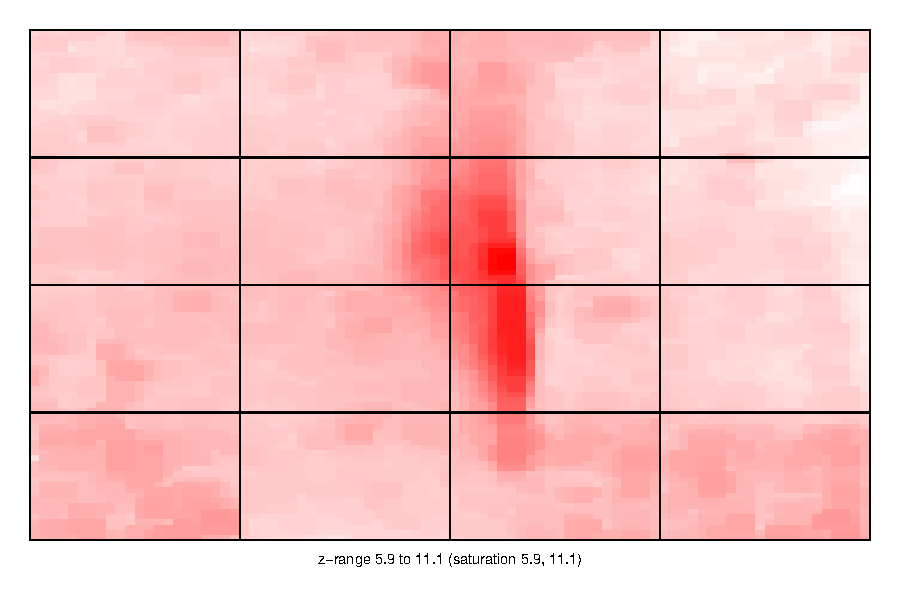
\includegraphics{plots/fig-019}
  \end{itemize}
\end{frame}

\begin{frame}[fragile, allowframebreaks]
  \frametitle{imageplot green}
\begin{Schunk}
\begin{Sinput}
> imageplot(log2(RG$Gb[, 1]), RG$printer, 
+     low = "white", high = "green")
\end{Sinput}
\end{Schunk}
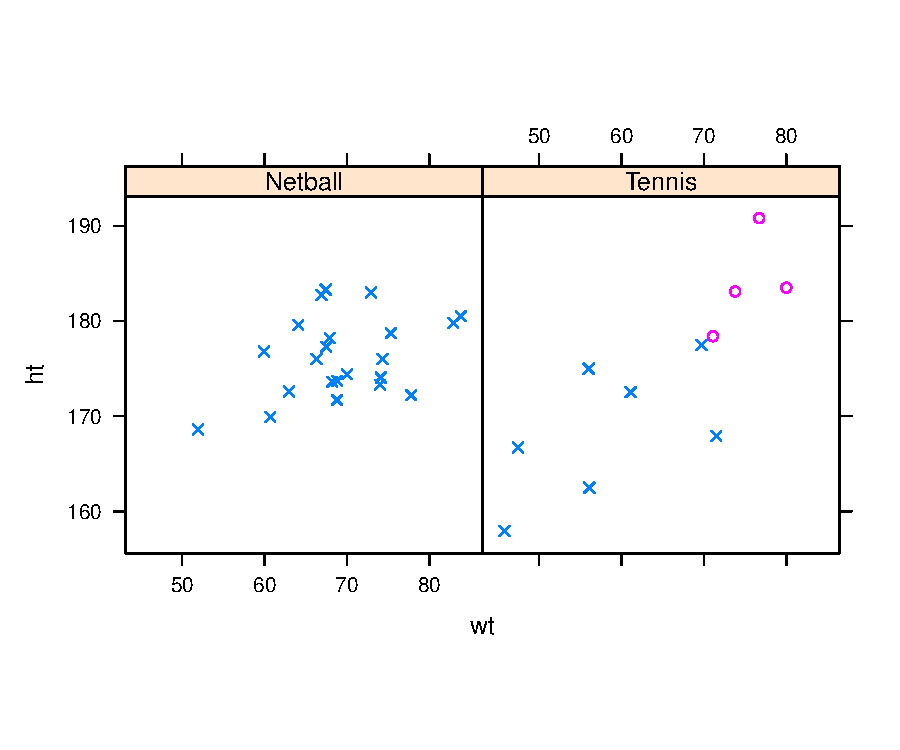
\includegraphics{plots/fig-020}
\end{frame}

\begin{frame}[allowframebreaks, fragile]
  \frametitle{normalizeWithinArrays}
  \begin{itemize}
  \item Just by looking at that first array we realized that we need to normalize the data.
  \item Using \BIOCfunction{normalizeWithinArrays} we can normalize the data using its \emph{log-ratio} such that the mean of these will be 0..
\begin{Schunk}
\begin{Sinput}
> MA <- normalizeWithinArrays(RG, 
+     method = "none")
\end{Sinput}
\end{Schunk}
  \item Lets check if we got a satisfying result: 
\begin{Schunk}
\begin{Sinput}
> imageplot(MA$M[, 1], RG$printer, 
+     zlim = c(-3, 3))
\end{Sinput}
\end{Schunk}
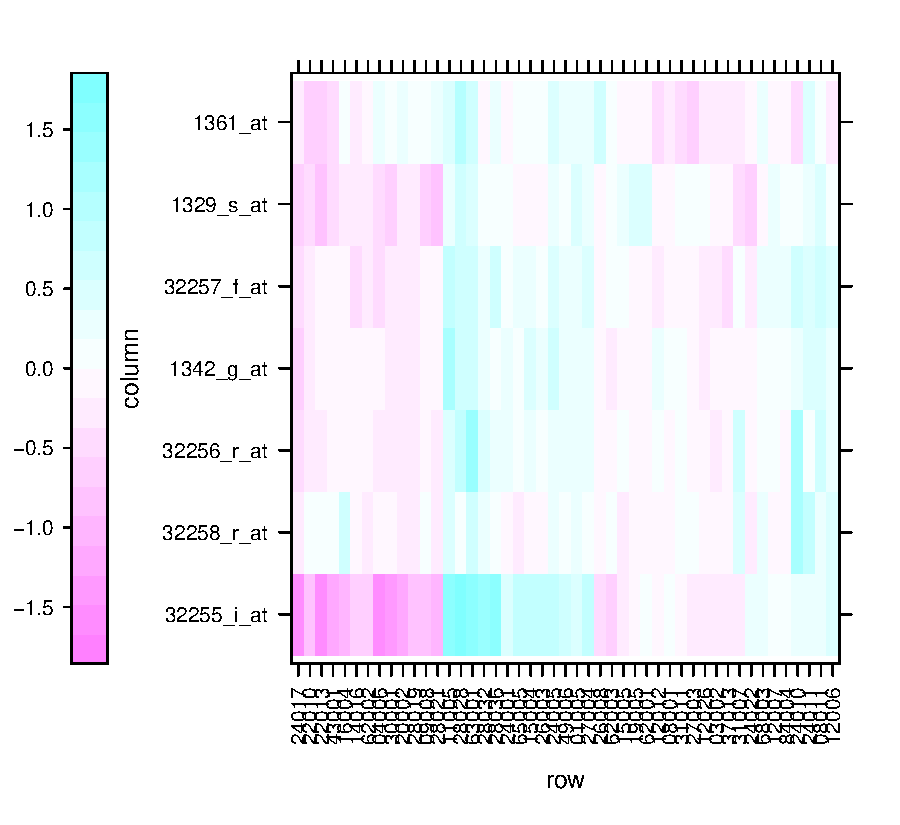
\includegraphics{plots/fig-022}
  \end{itemize}
\end{frame}

\begin{frame}[allowframebreaks]
  \frametitle{o\_O}
  \begin{itemize}
  \item The function \pl{imageplot} rotates the array, such that the group at the bottom left corner is the first one.
  \item In this last plot we observe a red line. Till tells us that there was some powder or that the microarray was damaged there.
  \item The data from that zone will have suspicious values.
  \end{itemize}
\end{frame}

\begin{frame}[allowframebreaks, fragile]
  \frametitle{plotMA}
  \begin{itemize}
  \item In microarrays, its useful to make a "MA" plot.
  \item In these, we plot the ratio R vs G versus the intensity of the point.
  \item The value $M$ is determined by:
  \begin{displaymath}M = log_{2}(R) - log_{2}(G)
  \end{displaymath}
  \item THe value $A$ represents the intensity and is given by:or:
  \begin{displaymath}
  A = (log_{2}(R) + log_{2}(G))/2
  \end{displaymath}
  \item We can make this kind of plot using \BIOCfunction{plotMA}.
\begin{Schunk}
\begin{Sinput}
> plotMA(MA)
\end{Sinput}
\end{Schunk}
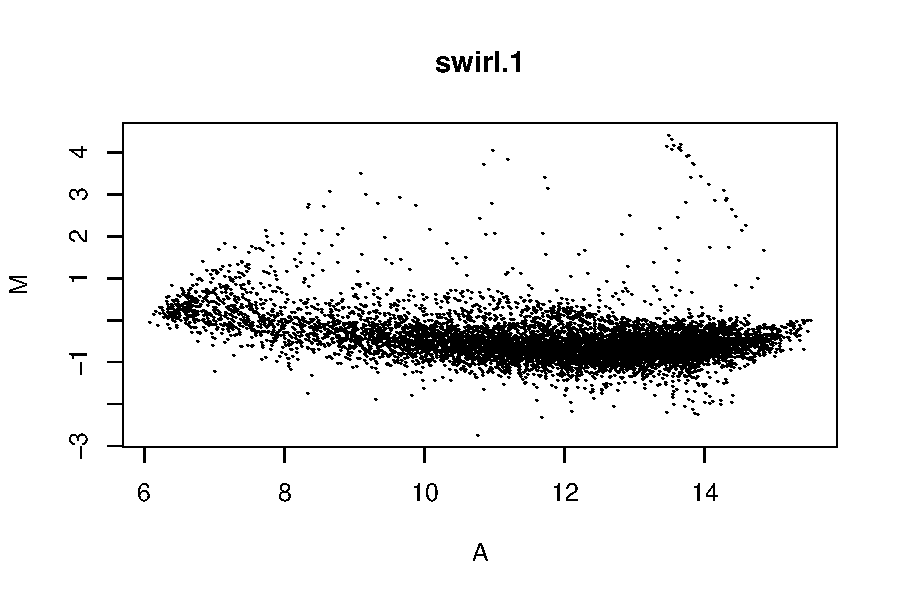
\includegraphics{plots/fig-023}
  \end{itemize}
\end{frame}

\begin{frame}[allowframebreaks, fragile]
  \frametitle{plotPrintTipLoess}
  \begin{itemize}
  \item In the previous plot we can see how the values derived from the damaged zone are in the top right hand corner.
  \item When we have lots of data, we need to deal with \emph{outliers}. That's why we use functions such as \BIOCfunction{lowess} and \BIOCfunction{loess}. \pl{lowess} makes a "locally weighted polynomial regression". Its older hence why it doesn't use the formula notation.
  \item We can use \BIOCfunction{plotPrintTipLoess} to visualize all the data from our first array and the loess curve which we'll use to normalize the data.
\begin{Schunk}
\begin{Sinput}
> plotPrintTipLoess(MA)
\end{Sinput}
\end{Schunk}
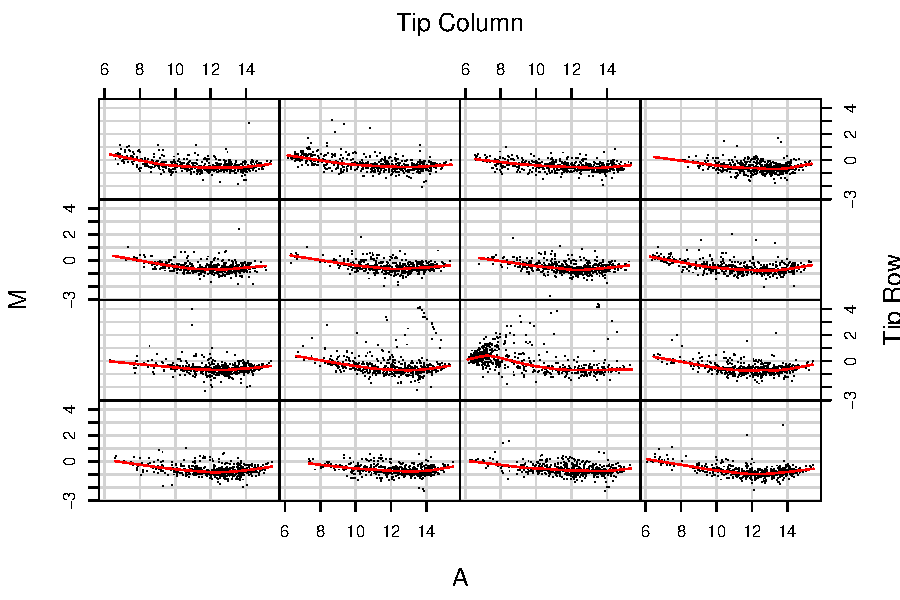
\includegraphics{plots/fig-024}
  \end{itemize}
\end{frame}

\begin{frame}[allowframebreaks, fragile]
  \frametitle{Normalizing}
  \begin{itemize}
  \item Now lets normalize the data using default params and lets look at the same plot again.
  \item In reality we are only normalizing the $M$ values for each array.
\begin{Schunk}
\begin{Sinput}
> MA <- normalizeWithinArrays(RG)
> plotPrintTipLoess(MA)
\end{Sinput}
\end{Schunk}
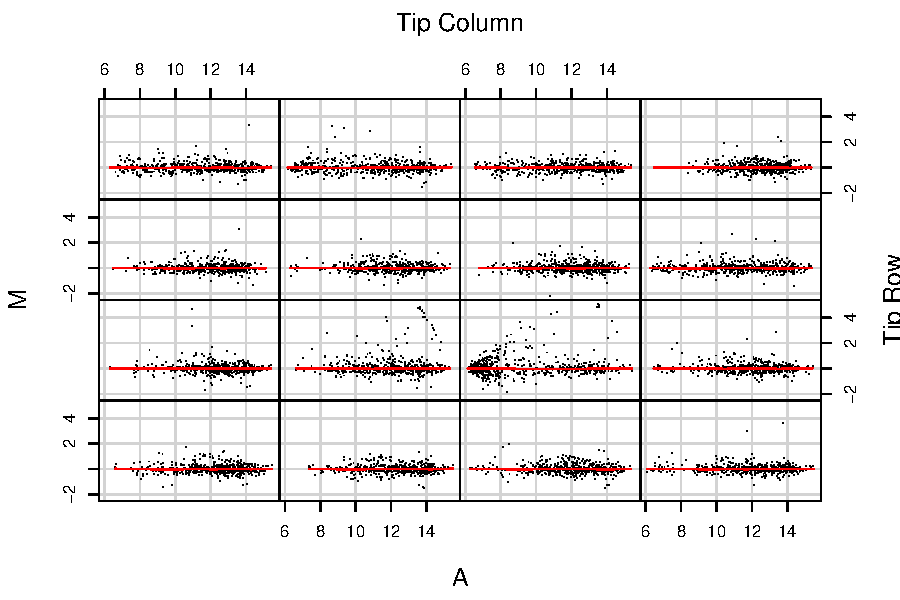
\includegraphics{plots/fig-025}
  \end{itemize}
\end{frame}

\begin{frame}[allowframebreaks, fragile]
  \frametitle{Between arrays?}
  \begin{itemize}
  \item Next we can ask ourselves if we need to normalize between the 4 microarrays.
  \item To do so, we'll use the basic \pl{R} function \pl{boxplot}:
\begin{Schunk}
\begin{Sinput}
> boxplot(MA$M ~ col(MA$M), names = colnames(MA$M))
\end{Sinput}
\end{Schunk}
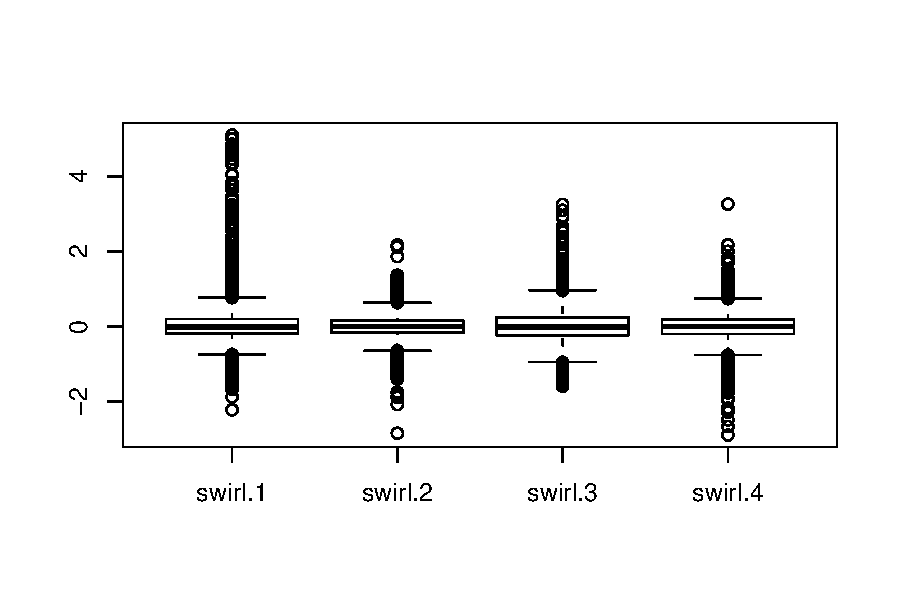
\includegraphics{plots/fig-026}
  \end{itemize}
\end{frame}

\begin{frame}[allowframebreaks, fragile]
  \frametitle{normalizeBetweenArrays}
  \begin{itemize}
  \item Because we can observe variation between the arrays, lets normalize them. Many times this is not necessary.
  \item Let use \BIOCfunction{normalizeBetweenArrays} with the default method and look at the result with \pl{boxplot}.
  \item The default method is \pl{Aquantile} which makes sure that the $A$ values have the same empirical distribution in the arrays without changing the $M$ values.
\begin{Schunk}
\begin{Sinput}
> MA <- normalizeBetweenArrays(MA, 
+     method = "scale")
> boxplot(MA$M ~ col(MA$M), names = colnames(MA$M))
\end{Sinput}
\end{Schunk}
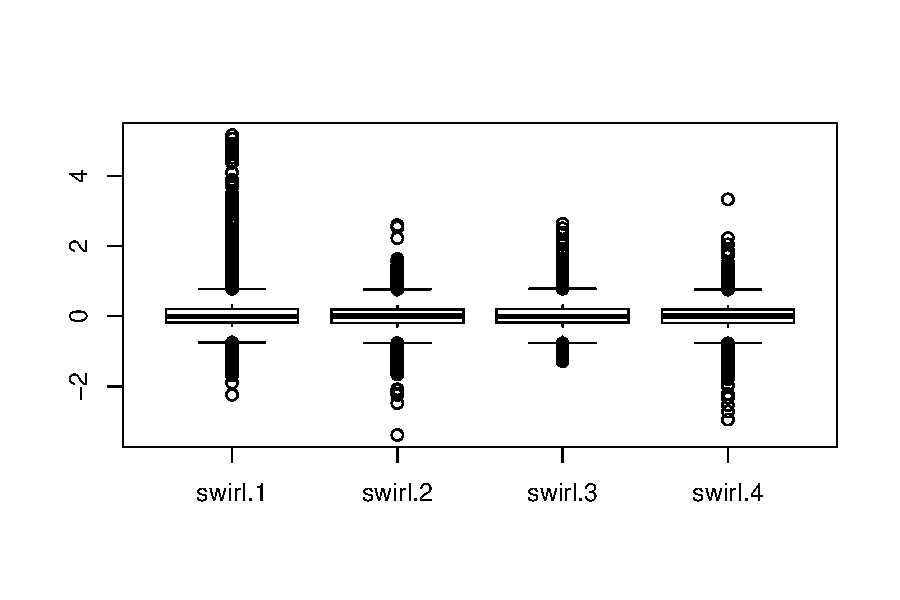
\includegraphics{plots/fig-027}
  \end{itemize}
\end{frame}

\begin{frame}[allowframebreaks, fragile]
  \frametitle{lmFit}
  \begin{itemize}
  \item Now we'll use a linear model to estimate (predict) the value $M$ for every gene.
  \item First we need to specify the experimental design; when every color was used:
\begin{Schunk}
\begin{Sinput}
> design <- c(-1, 1, -1, 1)
\end{Sinput}
\end{Schunk}
  \item Next we find our linear regression using the function \BIOCfunction{lmFit} which is especifically designed for microarrays.
\begin{Schunk}
\begin{Sinput}
> fit <- lmFit(MA, design)
\end{Sinput}
\end{Schunk}
  \item The resulting object has lots of information. Take a look!
\begin{Schunk}
\begin{Sinput}
> fit
\end{Sinput}
\end{Schunk}
  \end{itemize}
\end{frame}

\begin{frame}[allowframebreaks, fragile]
  \frametitle{$t$ tests}
  \begin{itemize}
  \item In our objet \pl{fit}, \pl{coefficients} is the mean $M$ value while \pl{sigma} is the standard deviation for each gene.
  \item We can now make $t$ tests to compare the mutant with the WT for every gene:
\begin{Schunk}
\begin{Sinput}
> ordinary.t <- fit$coef/fit$stdev.unscaled/fit$sigma
\end{Sinput}
\end{Schunk}
  \item Now we can make a plot with the mean $M$ and $A$ values for every gene:
\begin{Schunk}
\begin{Sinput}
> plotMA(fit)
> abline(0, 0, col = "blue")
\end{Sinput}
\end{Schunk}
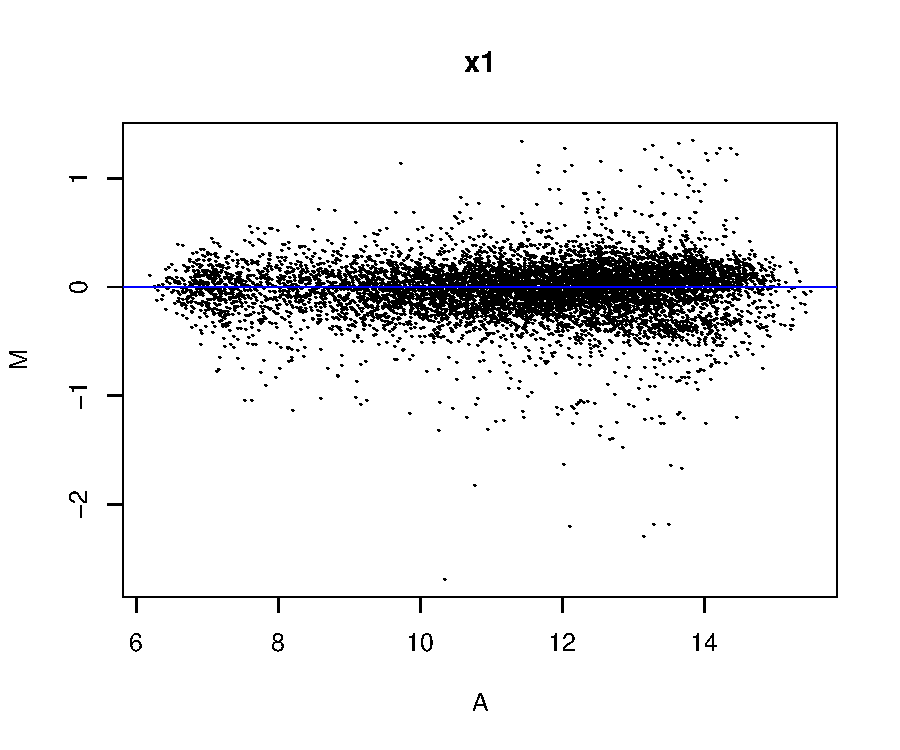
\includegraphics{plots/fig-032}
  \end{itemize}
\end{frame}

\begin{frame}[allowframebreaks, fragile]
  \frametitle{eBayes}
  \begin{itemize}
  \item According to the \pl{limma} creators, its better to use $t$ tests moderated with empirical Bayes; aka, using \BIOCfunction{eBayes}.
  \item With this we can find the differentially expressed genes.
  \item Actually, \pl{eBayes} uses the empirical Bayes estimation to minimize the standar errors towars a common value.
\begin{Schunk}
\begin{Sinput}
> fit <- eBayes(fit)
\end{Sinput}
\end{Schunk}
  \item Next, lets make a QQ plot to check if we have differentially expressed genes. Lets use \BIOCfunction{qqt} instead of \pl{qq} because we want to compare against the $t$ distribution quantiles and not versus a normal dist.
\begin{Schunk}
\begin{Sinput}
> qqt(fit$t, df = fit$df.prior + 
+     fit$df.residual, pch = 16, 
+     cex = 0.2)
> abline(0, 1)
\end{Sinput}
\end{Schunk}
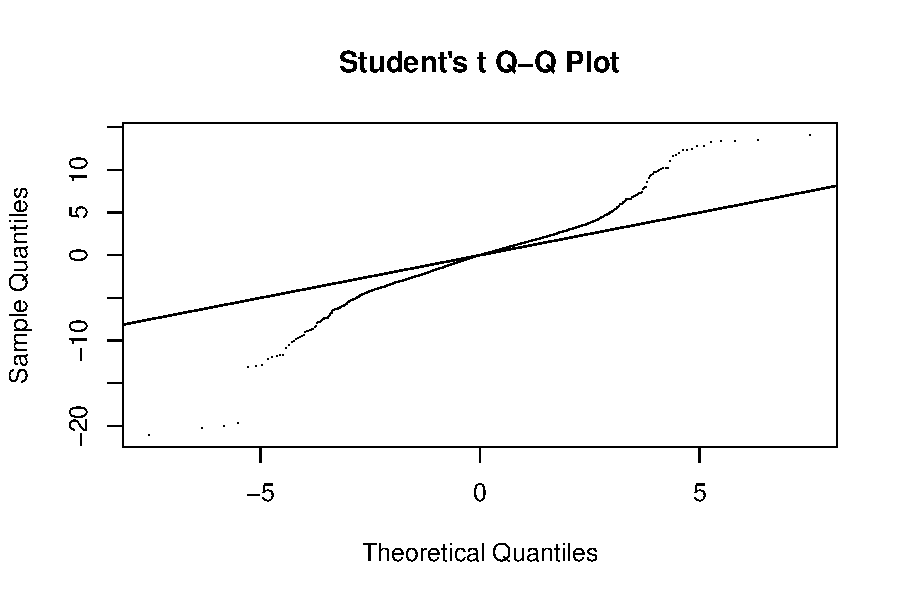
\includegraphics{plots/fig-034}
  \end{itemize}
\end{frame}

\begin{frame}[allowframebreaks, fragile]
  \frametitle{topTable}
  \begin{itemize}
  \item We have a lot of differentially expressed genes! :)
  \item To find which they are, we use the function \BIOCfunction{topTable}. An important argument is \pl{adjust.method}, because with it we specify how we want to correct our $p$ values.
  \item For example, with the following code you can look at the top 30 DEGs adjusting the $p$ values by FDR.
\begin{Schunk}
\begin{Sinput}
> topTable(fit, number = 30, adjust = "BH")
\end{Sinput}
\end{Schunk}
  \item I'll show you one:
\begin{Schunk}
\begin{Sinput}
> topTable(fit, number = 1, adjust = "BH")
\end{Sinput}
\begin{Soutput}
     Block Row Column      ID Name
3721     8   2      1 control BMP2
         logFC  AveExpr         t
3721 -2.205288 12.10451 -21.06952
          P.Value    adj.P.Val       B
3721 1.028468e-07 0.0003572816 7.96075
\end{Soutput}
\end{Schunk}
  \item As it was expected, our gene with the largest difference is BMP2. Remember that its knocked-out on the Swirl line.
  \item We can look at the original $p$ values, the adjusted ones, the \emph{log odds} from the empirtcal Bayes statistics, \ldots
  \end{itemize}
\end{frame}

\begin{frame}[allowframebreaks, fragile]
  \frametitle{Finishing with \pl{limma}}
  \begin{itemize}
  \item To finish our \pl{limma} practical session, lets mark the top 30 genes in our previous \pl{plotMA} plot.
  \item We'll use \BIOCfunction{order} and \BIOCfunction{text} from basic \pl{R} to do this.
\begin{Schunk}
\begin{Sinput}
> plotMA(fit)
> ord <- order(fit$lods, decreasing = TRUE)
> top30 <- ord[1:30]
> text(fit$Amean[top30], fit$coef[top30], 
+     labels = fit$genes[top30, "Name"], 
+     cex = 0.8, col = "blue")
\end{Sinput}
\end{Schunk}
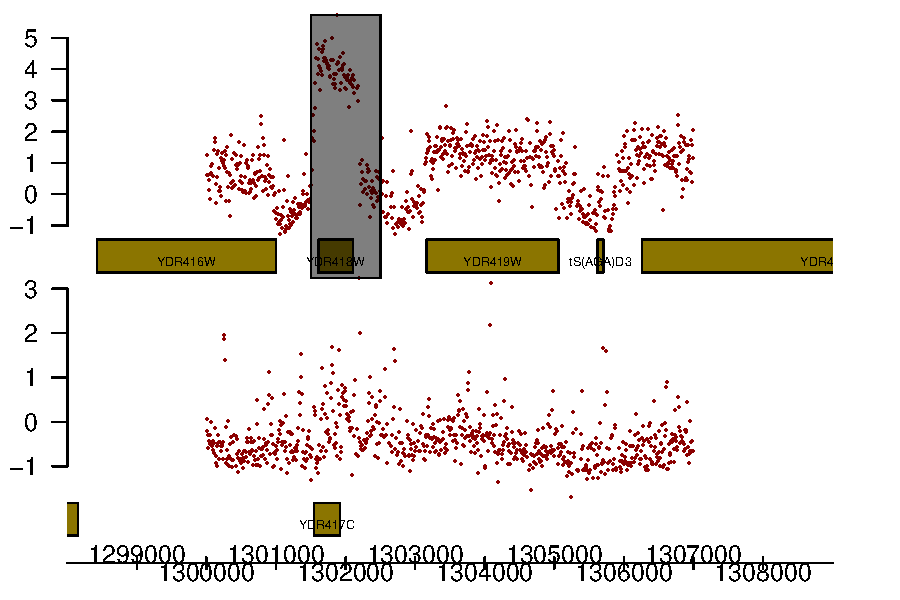
\includegraphics{plots/fig-037}
  \end{itemize}
\end{frame}

\section{Homework}
\begin{frame}[allowframebreaks]
  \frametitle{Homework}
  \begin{itemize}
  \item With a data set of your choice (but new!) that has two variables, make a plot with the linear regression.
  \item Calculate the Spearman and Pearson correlation coefficients.
  \item Add your own conclusions.
  \end{itemize}
\end{frame}

\begin{frame}[allowframebreaks, fragile]
  \frametitle{SessionInfo} \scriptsize
\begin{Schunk}
\begin{Sinput}
> sessionInfo()
\end{Sinput}
\begin{Soutput}
R version 2.10.0 Under development (unstable) (2009-07-21 r48968) 
i386-pc-mingw32 

locale:
[1] LC_COLLATE=English_United States.1252 
[2] LC_CTYPE=English_United States.1252   
[3] LC_MONETARY=English_United States.1252
[4] LC_NUMERIC=C                          
[5] LC_TIME=English_United States.1252    

attached base packages:
[1] stats     graphics  grDevices
[4] utils     datasets  methods  
[7] base     

other attached packages:
[1] limma_2.19.2  UsingR_0.1-12
\end{Soutput}
\end{Schunk}
\end{frame}

\end{document}

